\documentclass[tikz,border=2pt]{standalone}
\usepackage{amsmath,amssymb}
\usepackage{tikz}
\usetikzlibrary{arrows.meta}

\begin{document}
% Mixed constraints: an equality h(x) = c (the curve) and an inequality g(x) <= b (the
% half-plane); the feasible set is the arc of the curve inside the half-plane, and at the
% optimum grad f is a combination of grad h (any sign) and grad g (nonnegative, zero if slack).
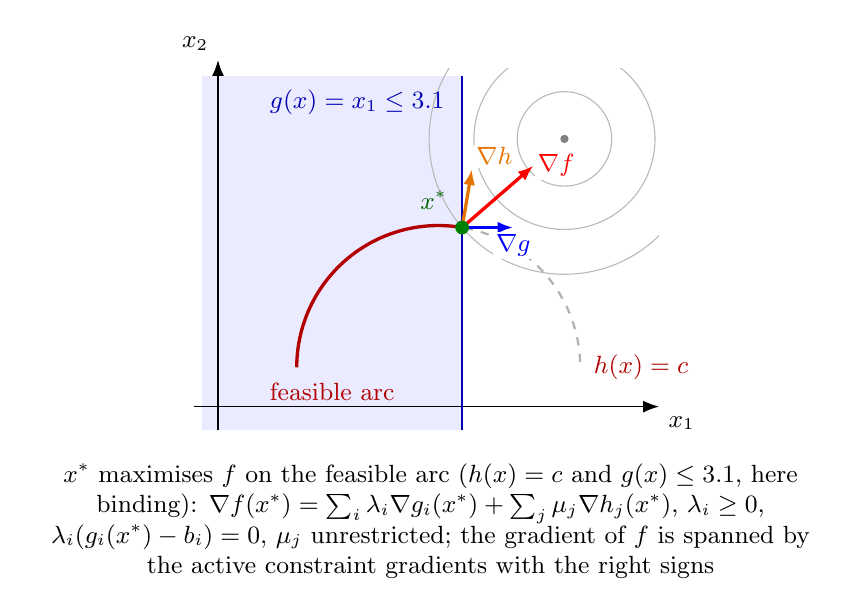
\begin{tikzpicture}[every node/.style={font=\small}, >={Latex[length=2mm]}, lab/.style={font=\small, fill=white, inner sep=1pt}]
	\fill[blue!8] (-0.2,-0.3) rectangle (3.1,4.2);
	\begin{scope}
		\clip (-0.2,-0.3) rectangle (5.6,4.3);
		\foreach \r in {0.6,1.15,1.719} {\draw[gray!55] (4.4,3.4) circle (\r);}
	\end{scope}
	\fill[gray] (4.4,3.4) circle (1.5pt);
	\draw[->] (-0.3,0) -- (5.6,0) node[below right] {$x_1$};
	\draw[->] (0,-0.3) -- (0,4.4) node[above left] {$x_2$};
	\draw[blue!70!black, thick] (3.1,-0.3) -- (3.1,4.2);
	\node[blue!70!black, anchor=north east, font=\small] at (3.0,4.15) {$g(x)=x_1\le3.1$};
	\draw[gray!60, thick, dashed] (1.0,0.5) arc (180:0:1.8);
	\draw[red!70!black, very thick] (1.0,0.5) arc (180:80.4:1.8);
	\node[red!70!black, anchor=west, font=\small] at (4.65,0.5) {$h(x)=c$};
	\node[red!70!black, font=\small, anchor=north] at (1.45,0.42) {feasible arc};
	\draw[->, red, very thick] (3.1,2.275) -- (4.007,3.06) node[right, lab] {$\nabla f$};
	\draw[->, blue, very thick] (3.1,2.275) -- (3.75,2.275) node[below, lab, yshift=-1pt] {$\nabla g$};
	\draw[->, orange!90!black, very thick] (3.1,2.275) -- (3.225,3.015) node[above right, lab] {$\nabla h$};
	\fill[green!50!black] (3.1,2.275) circle (2.5pt);
	\node[green!40!black, anchor=south east, font=\small] at (3.03,2.38) {$x^\ast$};
	\node[anchor=north, align=flush center, text width=10cm] at (2.7,-0.6) {$x^\ast$ maximises $f$ on the feasible arc ($h(x)=c$ and $g(x)\le3.1$, here binding): $\nabla f(x^\ast)=\sum_i\lambda_i\nabla g_i(x^\ast)+\sum_j\mu_j\nabla h_j(x^\ast)$, $\lambda_i\ge0$, $\lambda_i(g_i(x^\ast)-b_i)=0$, $\mu_j$ unrestricted; the gradient of $f$ is spanned by the active constraint gradients with the right signs};
\end{tikzpicture}
\end{document}
